% !TEX root = ../notes_template.tex
\chapter{Muscle Regulation}\label{chp:regulation}
Updated on \today
\minitoc

Understanding the mechanisms of muscle activation and excitation enables an understanding regulation. All of these terms are referring to active tension - the activation of active tension, the excitation that results in activation of active tension, and the regulation of the excitations that result in active tension. A single excitation produces enough activation to create a twitch, making a twitch the fundamental unit of active tension. Regulation of active tension involves the mechanisms that are utilized to allow a muscle fiber, and the muscle, to vary its active tension from (essentially) zero to its maximal value. For voluntary movement the regulation of active tension must be accurate and precise. This requires activation to start and stop when needed (events involving EAC and Ca+ release and uptake by the SR). And it requires excitation to start and stop when needed (events involving rapid depolarization and repolarization of excitable membranes). Regulation of active tension includes the processes used by the central nervous system to vary its active tension from the lowest value (resting tone) to its maximal value (maximal voluntary contraction (MVC)). 




Excitation occurs for an entire The regulation of active tension is managed by the central nervous system. This chapter introduces the mechanisms utilized by the CNS to fulfill this role. The CNS has one approach for muscle fiber tension regulation - it can manipulate the number of twitches per second (frequency summation); and one approach for whole muscle tension regulation - it can manipulate the number of muscle fibers twitching (motor unit summation). 

\vspace{5mm}

\textbf{Objectives include:}
\begin{enumerate}
    \item Explain motor unit structure–function relationships.
    \item Explain muscle fiber differentiation structure-function relationships.
    \item Explain motor unit excitation, twitch and tetany.
    \item Explain motor unit summation and the order of recruitment.
    \item Explain the effect of multiple sclerosis on motor unit excitation.
    \item Explain how the muscle spindles and the golgi tendon organs influence motor unit excitation.
    \item Explain the physiological basis of the electromyogram (EMG) and limitations of EMG interpretation.
    \item Explain the effect of amyotrophic lateral sclerosis and aging on motor units.
\end{enumerate}\

\section{Motor Units}

A motor unit is an $\alpha$-motor neuron and all of muscle fibers that its terminal axon branches form a neuromuscular junction at a motor end plate. Each muscle fiber has one motor end plate, and therefore one neuromuscular junction. However, each $\alpha$-motor neuron has many terminal axon branches. 

\begin{figure}[!ht]
    \centering
    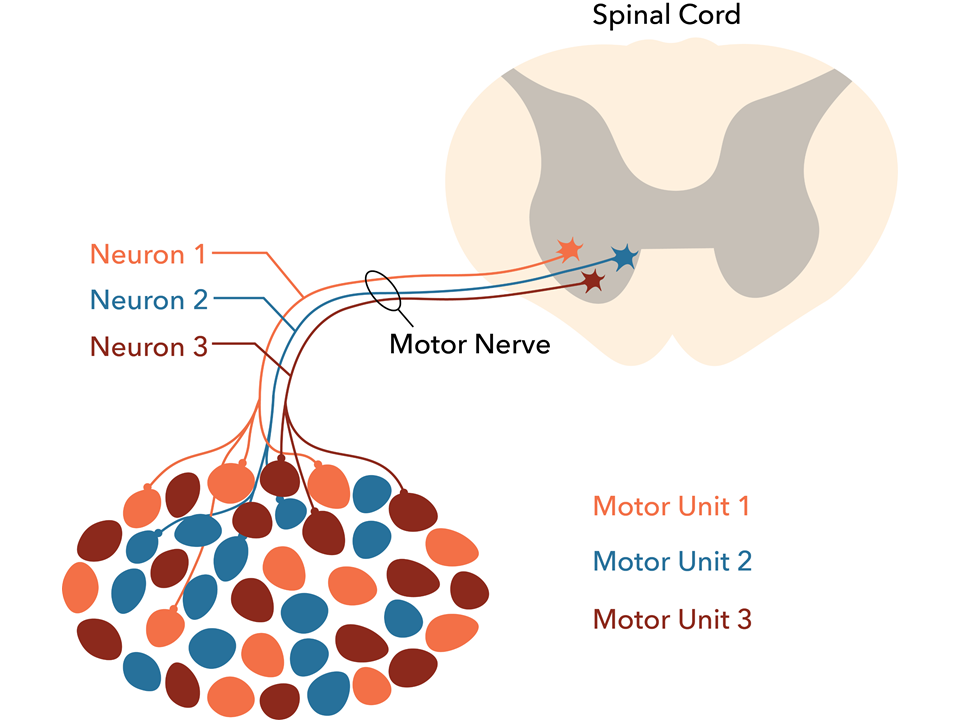
\includegraphics[width=1\linewidth]{./figure/motor_unit.png}
    \caption{Motor Unit Distribution in a Muscle \footnotesize{\href{https://commons.wikimedia.org/wiki/File:Motor_unit.png}{Wikimedia Commons, CC BY 4.0})}}
    \label{fig:motor_unit}
\end{figure}




\subsection{Motor Unit Types}

There are three motor unit types using a classification based on measurements on motor unit twitch tension, twitch time and fatigue index (See Table \ref{table:Motor_Unit_Types}.

% Diameters from 12 - 22 \mu m 

\begin{table}[h!]
\centering
\begin{tabular}{||c c c c||} 
 \hline
 Motor Unit Type & Twitch Tension & Twitch Time & Fatigue Index \\ [0.5ex] 
 \hline\hline
 Fast-Fatigable (FF)  & High & Fast & Low \\ 
 Fast-Resistant (FR)  & Moderate & Fast & Moderate \\
 Slow (S) &  Low & Slow & High \\ [1ex] 
 \hline
\end{tabular}
\caption{Motor Unit Types}
\label{table:Motor_Unit_Types}
\end{table}


\subsection{Muscle Fiber Types}


\begin{table}[h!]
\centering
\begin{tabular}{||c c c c ||} 
 \hline
Characteristic & Type 1 / SO & Type 2x / FOG & Type 2a / FG \\ 
 \hline\hline
 Fatigue Resistant & FF & Fast & Low \\ 
 Shortening Velocity & FR & Fast & Moderate \\
  & S & Slow & High \\ [1ex] 
 \hline
\end{tabular}
\caption{Muscle Fiber Types}
\label{table:Motor_Unit_Types}
\end{table}


\section{Motor Unit Excitation}

An $\alpha$-motor neuron, once excited, will release only one neurotransmitter, ACh at its axon terminal. ACh will only have one effect at the NMJ, creating excitatory micro-potentials on the motor end plate. However, in the Central Nervous System (such as the Spinal Cord) competing neurotransmitters can be released at synapses of the $\alpha$-motor neuron dendrites. The impact of these neurotransmitters can be excitatory or inhibitory. Since they occur after the synaspse they are called excitatory post synaptic potentiations (EPSPs) or inhibitory post synaptic potentiations (IPSPs). Whether, and how frequently, an $\alpha$-motor neuron sends an excitation to the muscle fibers it innervates is balanced by competition between the EPSPs and the IPSPs.



\subsection{Motor Unit Twitch}

Difference between motor unit twitch $T_{mu}$ and muscle fiber twitch $T_{mf}$


\begin{equation}
    T_{mu} = N_ \cdot T_{mf} = N \cdot A \cdot T_s
\end{equation}

$N$ refers to the number of muscle fibers and in the above equation since there is only one motor unit being considered N can be taken as the the innervation ratio (IR)

$A$ refers to the cross sectional area - an indication of how many sarcomeres are in parallel in the fiber

$T_s$ refers to the tension created for each unit of cross sectional area

$IR = \frac{N_{mf}}{N_{mu}}$ (Note, when there is one motor unit, $N = IR = N_{mf}$)

Why is there more tension in a FF motor unit excitation and FG muscle fiber twitch? Three reasons: first, because there are more muscle fibers in a FF motor unit ($N_{mf}$). Second, because the muscle fibers in the FF motor unit have greater cross sectional area ($A$). Third, and to a much lesser extent, because the sarcomeres of a FG muscle fiber create more tension per twitch even when controlling for $A$ ($T_s$) \cite{bodine_maximal_1987}. Although this third reason remains controversial due to the small difference between the $T_s$ of FG and SO muscle fibers \cite{lieber_skeletal_2010}. Some sources equate the $T_s$ between the two fiber types, $T_s \simeq 20 N \cdot cm^{-2}$ \cite{feher_quantitative_2017}, whereas others report them separately with albeit different estimates, FG $T_s \simeq 22 N \cdot cm^{-2}$, and SO $T_s \simeq 15 N \cdot cm^{-2}$ \cite{lieber_skeletal_2010}.


% Make more tables - make a table with the parameters of the equation including N, A, Fs for estimates of Fmu




\subsection{Motor Unit Tetany - Frequency Summation}

Rate coding

% Add the impact of multiple sclerosis on nerve conduction velocity (NCV) and the impact on NCV on regulation




\subsection{Motor Unit Summation - Recruitment}

\begin{figure}[!ht]
    \centering
    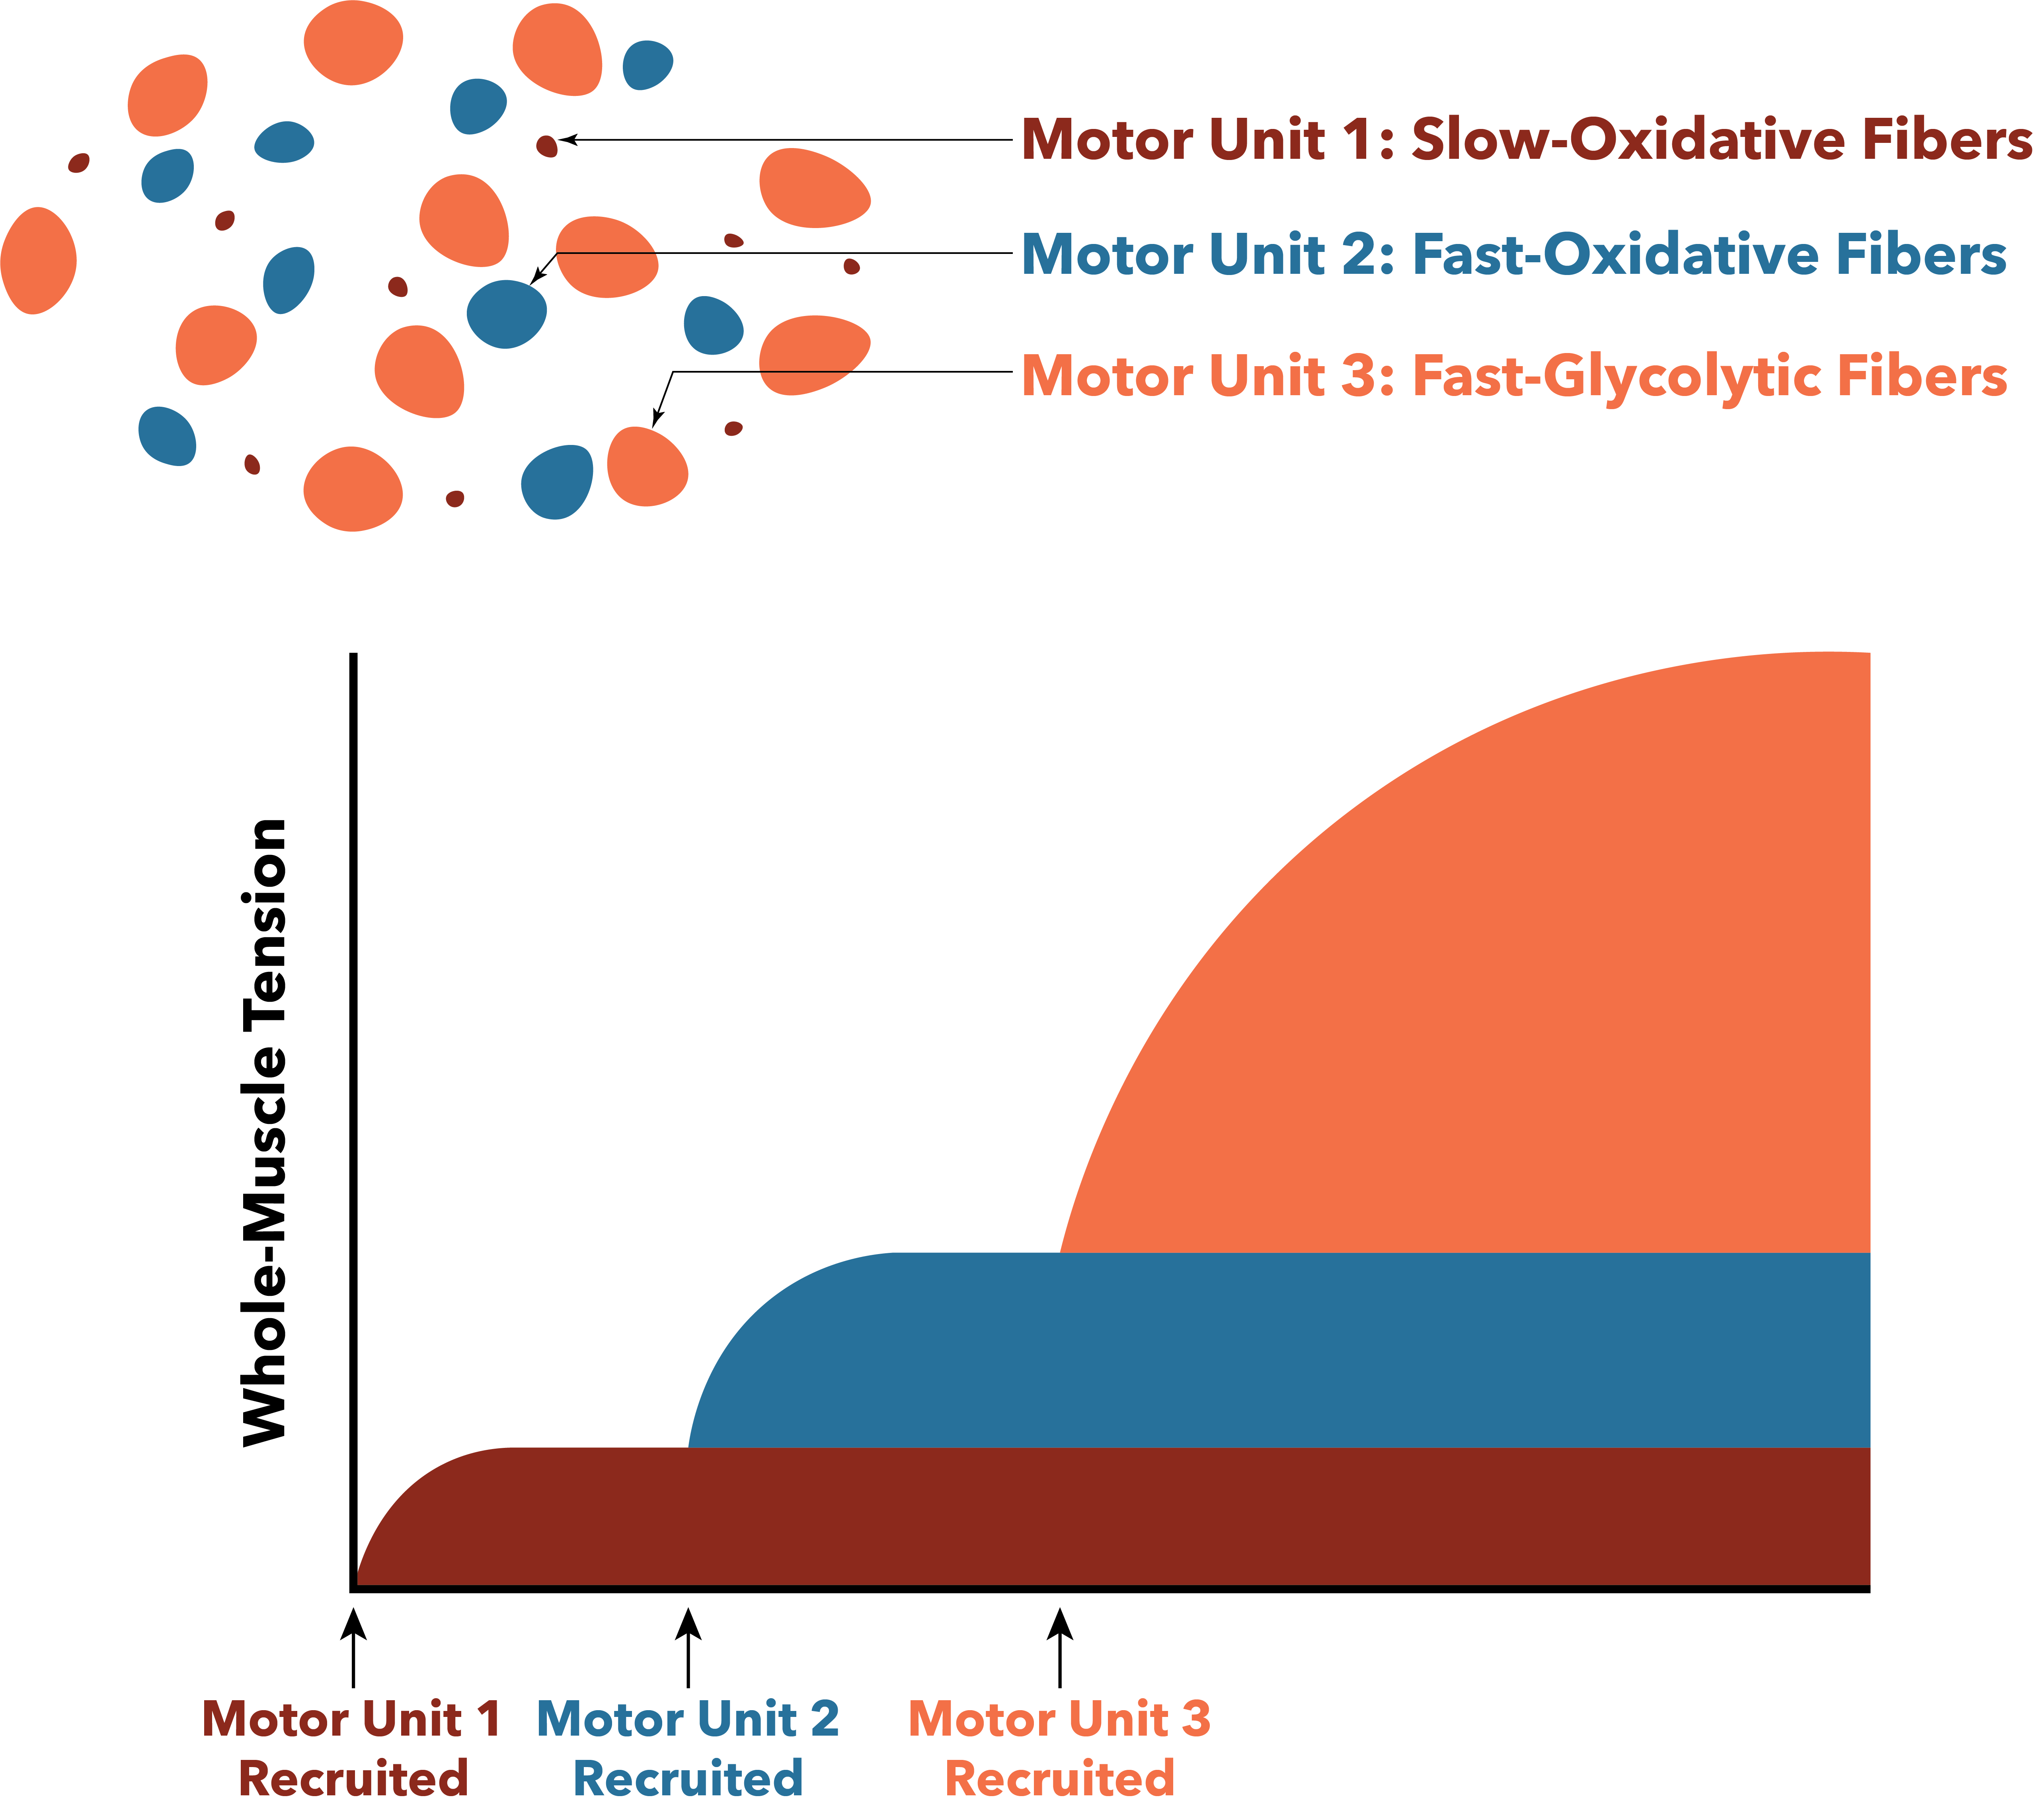
\includegraphics[width=1\linewidth]{./figure/Motor_unit_recruitment.png}
    \caption{Order of Recruitment \footnotesize{\href{https://commons.wikimedia.org/wiki/File:Motor_unit_recruitment.png}{Wikimedia Commons, CC BY 4.0})}}
    \label{fig:Motor_unit_recruitment}
\end{figure}

% Synchronous vs. asynchronous activation of multiple motor units

\section{Regulatory Feedback}

It is estimated that between 40\% to 70\% of the nerves in a nerve bundle to a skeletal muscle fiber are $\alpha$-motor neurons (\underline{e}fferent nerves, \underline{e}xiting the spinal cord). The remaining axons are from sensor nerves (\underline{a}fferent nerves, \underline{a}ccessing the spinal cord). Regulation of tension is critically dependent on knowing whether the intention of tension is being met (whatever that intention may be) so that tension can be adjusted as necessary. Since neither motor control or neuroscience is a focus of this book (or course) this section is brief and focused on the muscle spindles and golgi tendon organs (GTOs) and how they influence tension regulation in the the spinal cord. 

\subsection{Muscle Spindles}

Muscle spindles are receptors that are excited when stretched and provide the central nervous system with information about muscle length and rate of stretching. With this information the muscle spindles are important contributors to proprioception (sensation and perception of position and movement). They are located within fascicles along side (parallel to) muscle fibers. It is conventional, once speaking of the muscle spindle, to refer to muscle fibers as extrafusal fibers (not part of the muscle spindle). The muscle spindles have both afferent and efferent innervation and their own small set of intrafusal contractile fibers. The intrafusal fibers are innervated by $\gamma$-motor neurons and allow the muscle spindle to adjust to the length of the muscle to remain sensitive to changes in length (See Figure \ref{fig:MuscleSpindle}). 

\begin{figure}[!ht]
    \centering
    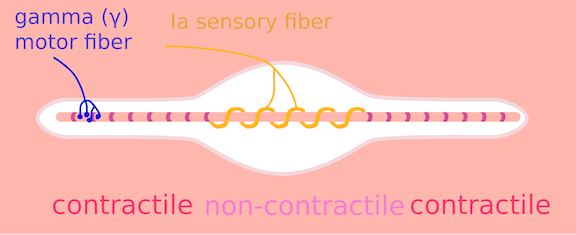
\includegraphics[width=1\linewidth]{./figure/MuscleSpindle.png}
    \caption{Muscle Spindle \footnotesize{\href{https://commons.wikimedia.org/wiki/File:MuscleSpindle.svg}{Wikimedia Commons, CC BY 4.0})}}
    \label{fig:MuscleSpindle}
\end{figure}

Afferent signals from the muscle spindles terminate at the spinal cord as well as higher up in the central nervous system for long loop reflexes and coordination (cerebellum) and the cerebral cortex (proprioception). The response of muscle spindles to a rapid increase in length (quick stretch) signals the dendrites of the $\alpha$-motor neurons of the agonist (same muscle that is being stretched) with excitatory post synaptic potentiations (EPSPs); and the dendrites of the $\alpha$-motor neurons of the antagonist (opposite muscles of those that are being stretched) with inhibitory post synaptic potentiations (IPSPs). Collectively these actions are referred to as the stretch reflex. If the stretch is quick enough and excites enough muscle spindles the EPSPs are sufficient enough to excite $\alpha$-motor neurons which provoke muscle excitation and activation. Testing stretch reflexes are an important component of a physical exam when the integrity of the $\alpha$-motor neuron is in question.

\subsection{Golgi Tendon Organs}

Golgi tendon organs (GTOs) are on the mostly tendon side of the transition space known as the musculotendinous junction. They are so close to muscle fibers that each GTO is connected in series with 5-20 muscle fibers. In this position the GTOs are detect tension in muscle and tendinous fibers \cite{macefield_physiological_2005}. The GTO is excited by tension within the muscle fibers or tendon. Afferent impulses from the GTOs terminate in the spinal cord and cerebellum. GTO afferents in the spinal cord results in IPSPs of the agonist muscle. Inhibiting the agonist limits active tension as a protective mechanism.

\section{\textit{Clinical Physiology Connections}}

\subsection{Electromyogram (EMG)}

Each time a muscle fiber is activated it is caused by an action potential from the nerve to the motor end plate, and along the sarcolemma of all the fibers that are innervated by that $\alpha$-motor neuron. Therefore, each muscle fiber activation is associated with an electrical signal. An EMG electrode near the fiber can record this electrical activity. The electrode can either be a small needle that acts as an antenna to record local electrical activity or a surface electrode (sEMG). If using a needle, the raw EMG signal can be used to accurately determine when a particular muscle is active (regardless of depth or size of the muscle). sEMG can be used to determine when a particular muscle is active when the muscle of interest is superficial and large enough to avoid cross talk at the sEMG electrode. 

\paragraph{EMG quantification} It is difficult to quantify the activity of a muscle from a raw EMG signal. The EMG contains electrical signals from every muscle fiber in the vicinity of the EMG electrode which creates a very noisy signal (See Figure \ref{fig:EMG_ARV}. From the raw signal the Average Rectified Voltage (ARV) EMG can be computed. ARV is a time-windowed mean of the absolute value of the signal (turns all voltages into positive values). ARV is useful for further analysis such as recording the excitation patterns of a muscles that may include changes in excitation or as the first step towards more advanced analyses \cite{merletti_surface_2016}. The relationship between EMG activity and muscle tension is most valuable during isometric activation because the association between activation and tension changes with changes in length (length-tension relationship), and with different velocities (force-velocity relationship).

\begin{figure}[!ht]
    \centering
    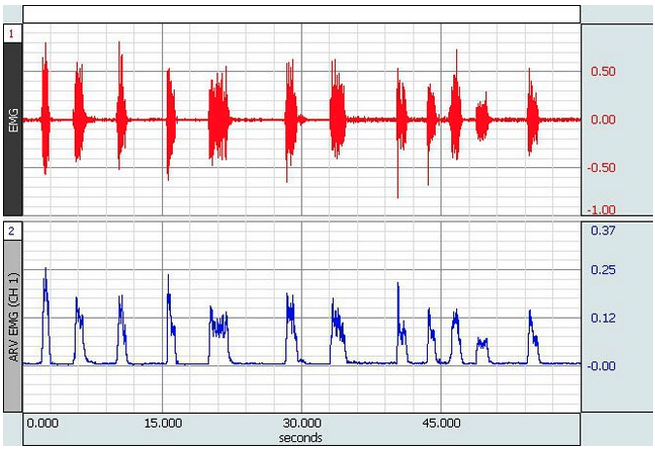
\includegraphics[width=1\linewidth]{./figure/EMG_ARV.png}
    \caption{Raw (upper) and ARV EMG Signals \footnotesize{Data collected using Biopaq acquisition hardware and Acknowledge software in the author's lab (SC)}}
    \label{fig:EMG_ARV}
\end{figure}

\paragraph{Biofeedack}

sEMG is a valuable form of biofeedback to indicate that a certain muscle has been activated. Commercially available devices provide visual or auditory signals so a patient can learn to activate a muscle. Common applications of the EMG for biofeedback is activation in the vastus medialis after anterior cruciate ligament surgery, or the lower trapezius during shoulder flexion or abduction.

\paragraph{Motor Unit Number and Size Indices (MUNIX \& MUSIX)}

The motor unit number index (MUNIX) and the motor unit size index (MUSIX) are based on sEMG data interpreted through a mathematical model to estimate an index of the number and size of functional $\alpha$-motor neurons for a muscle \cite{nandedkar_motor_2004}. MUNIX is not an absolute count of motor units, and MUSIX is not an absolute size of the motor units. But they do provide an estimate that correlates with other measures and they have reasonable reliability. Considering the test only takes 3-5 minutes per muscle, is non-invasive and relatively comfortable (as compared to other approaches), they have gained popularity in clinical neurology and neurophysiology. MUNIX is considered an effective bio-marker for assessing disease progression and an alternative clinical trial outcome in amyotrophic lateral sclerosis (ALS). It has also been proposed for use in the evaluation of peripheral neuropathies, particularly in demyelinating neuropathies with conduction block. While there have been less studies, MUNIX is starting to be evaluated in a variety of central nervous system disorders (such as spinal cord injury, stroke, and cerebral palsy \cite{fatehi_utility_2018}. 

A study of healthy individuals between 20 and 80 years of age demonstrated a reduction in MUNIX and MUSIX values with aging, particularly over the age of 60, indicating that they may be a valuable biomarker for research on the prevention and treatment of age related sarcopenia \cite{cao_reference_2020}. Sarcopenia is an age-related progressive loss of muscle mass and strength. It is a type of muscle atrophy primarily caused by the aging process and certainly confounded by physical inactivity and malnutrition. If a loss of motor units is inevitable with aging, then healthy aging would strive for lifestyles that promote increasing MUSIX despite an inevitable decline in MUNIX. A consequence of this shift (reduced MUNIX and increased MUSIX) would be a reduction in muscle tension regulation. Therefore, the choice of lifestyle would need to consider the motor control (balance, coordination) capabilities in such individuals.

\subsection{Nerve Conduction Velocity (NCV)}

Nerve conduction velocity (NCV) refers to the time it takes for an excitation to travel a certain distance. It can be measured clinical with electrodiagnostic testing that includes EMG. A stimulus is presented proximally at a peripheral nerve and the distal muscle excitation (via EMG) or axonal excitation is measured. NCV is related to the size of the neuron (diameter) because diameter influences resistance to current (flow of electrical impulses and therefore directly related to velocity). Diameter is inversely proportional to resistance, and resistance is inversely proportional to current, therefore diameter is directly proportional to current and velocity. The large diameter of the $\alpha$-motor neurons, combined with the myelin sheaths (See Figure \ref{fig:Motoneuron}, ensure a high NCV. 

Table \ref{table:NCV} shows the estimated NCV for three nerve fiber types. The $\alpha$-motor neuron has the highest NCV. The variation in diameter in these motor neurons is partially explained by the motor unit types with FF motor units innervating FG fibers having the larger diameter ($\simeq 22 \mu m$) on the higher end for NCV ($\simeq 120 m \cdot s^{-1}$), and the S motor units with the small diameters ($\simeq 12 \mu m$)and the lower end of NCV ($\simeq 70 m \cdot s^{-1}$).

\begin{table}[h!]
\centering
\begin{tabular}{||c c c c ||} 
 \hline
Nerve Fiber & Diameter (\mu m) & NCV ($m \cdot s^{-1}$) & Function \\ 
 \hline\hline
 $\alpha$-motor & 12-22 & 70-120 & motor \\ 
 $\delta$-sensory & 1-5 & 12-30 & sharp pain \\
 C & 0.5-1.2 & 0.2-2 & dull pain \\ [1ex] 
 \hline
\end{tabular}
\caption{NCV for different nerve fiber types \footnotesize{Note: C fibers are unmyelinated, whereas $\alpha$-motor and $\delta$-sensory fibers are myelinated. Therefore, C fibers have a larger drop in NCV estimated just from diameter.}}
\label{table:NCV}
\end{table}

The tight regulation of active tension for coordinated movements requires for fidelity in the signals coming from the central nervous system.\footnotemark\footnotetext{Fidelity in this context means that intended signals are accurately sent where and when they are requested.} If the myelin sheath of an $\alpha$-motor neuron is damaged the NCV is reduced. If the NCV is reduced then the ability to activate muscles with high fidelity signals is impaired resulting in delays in the generation of active tension, limiting the ability to increase active tension when needed. These changes occur for two reasons, first, limitations in frequency summation, and second, limitations in motor unit summation. This is precisely what happens in peripheral demyelinating diseases such as Guillain-Barre syndrome, Chronic Inflammatory Demyelinating Polyradiculoneuropathy, Anti-Myelin Associated Glycoprotein Neuropathy, and demyelinating disease known as Multiple Sclerosis also impairs signal fidelity, however, it is a central nervous system condition. Therefore, the loss of signal fidelity does not directly alter the peripheral NCV, it impairs the central NCV which interrupts signals that excite the motor unit dendrites in the spinal cord which tends to present as a more complicated, nuanced and variable clinical presentation (in terms of the impact it can have on motor function such as coordination).

\printbibliography[heading=subbibintoc]